\documentclass[journal]{IEEEtran}
\usepackage[a5paper, margin=10mm]{geometry}
%\usepackage{lmodern} % Ensure lmodern is loaded for pdflatex
\usepackage{tfrupee} % Include tfrupee package


\setlength{\headheight}{1cm} % Set the height of the header box
\setlength{\headsep}{0mm}     % Set the distance between the header box and the top of the text


%\usepackage[a5paper, top=10mm, bottom=10mm, left=10mm, right=10mm]{geometry}

%
\setlength{\intextsep}{10pt} % Space between text and floats

\makeindex


\usepackage{cite}
\usepackage{amsmath,amssymb,amsfonts,amsthm}
\usepackage{algorithmic}
\usepackage{graphicx}
\usepackage{textcomp}
\usepackage{xcolor}
\usepackage{txfonts}
\usepackage{listings}
\usepackage{enumitem}
\usepackage{mathtools}
\usepackage{gensymb}
\usepackage{comment}
\usepackage[breaklinks=true]{hyperref}
\usepackage{tkz-euclide} 
\usepackage{listings}
\usepackage{multicol}
\usepackage{xparse}
\usepackage{gvv}
%\def\inputGnumericTable{}                                 
\usepackage[latin1]{inputenc}                                
\usepackage{color}                                            
\usepackage{array}                                            
\usepackage{longtable}                                       
\usepackage{calc}                                             
\usepackage{multirow}                                         
\usepackage{hhline}                                           
\usepackage{ifthen}                                               
\usepackage{lscape}
\usepackage{tabularx}
\usepackage{array}
\usepackage{float}
\usepackage{ar}
\usepackage[version=4]{mhchem}


\newtheorem{theorem}{Theorem}[section]
\newtheorem{problem}{Problem}
\newtheorem{proposition}{Proposition}[section]
\newtheorem{lemma}{Lemma}[section]
\newtheorem{corollary}[theorem]{Corollary}
\newtheorem{example}{Example}[section]
\newtheorem{definition}[problem]{Definition}
\newcommand{\BEQA}{\begin{eqnarray}}
\newcommand{\EEQA}{\end{eqnarray}}

\theoremstyle{remark}


\begin{document}
\bibliographystyle{IEEEtran}
\onecolumn

\title{4.7.13}
\author{INDHIRESH S- EE25BTECH11027}
\maketitle


\renewcommand{\thefigure}{\theenumi}
\renewcommand{\thetable}{\theenumi}

\textbf{Question}.   Find the distance between the lines $l_1$ and $l_2$ given by
\begin{align*}
    \overrightarrow{r}=\hat{i}+2\hat{j}-4\hat{k}+\lambda(2\hat{i}+3\hat{j}+6\hat{k})\\\overrightarrow{r}=3\hat{i}+3\hat{j}-5\hat{k}+\mu(2\hat{i}+3\hat{j}+6\hat{k})
\end{align*}
\textbf{Solution}:\\
Let us solve the given equation theoretically and then verify the solution computationally. \\
Given equation:
\begin{align}
   \Vec{r}=\hat{i}+2\hat{j}-4\hat{k}+\lambda(2\hat{i}+3\hat{j}+6\hat{k}) \\
\Vec{r}=3\hat{i}+3\hat{j}-5\hat{k}+\mu(2\hat{i}+3\hat{j}+6\hat{k})\\
\end{align}
From the above two equation it is clear that given two lines are parallel.\\
Now we'll find the distance between them.\\
The given lines are in the form:
\begin{align}
   \Vec{r} = \myvec{1\\2\\-4} + k_1\myvec{2\\3\\6}\\
   \Vec{r} = \myvec{3\\3\\-5}+ k_2\myvec{2\\3\\6}
\end{align}
Where,
\begin{align}
    \Vec{A}=\myvec{1\\2\\-4}\;\;\,\Vec{B}=\myvec{3\\3\\-5}\;\;,\Vec{M}=\myvec{2&2\\3&3\\6&6}
\end{align}
From Least squares solution,for shortest distance:
\begin{align}
    \Vec{M^T}\Vec{M}\myvec{k_1\\-k_2}=\Vec{M^T}(\Vec{B}-\Vec{A})
\end{align}
\begin{align}
    \myvec{2&3&6\\2&3&6}\myvec{2&2\\3&3\\6&6}\myvec{k_1\\-k_2}=\myvec{2&3&6\\2&3&6}\brak{\myvec{3\\3\\-5}-\myvec{1\\2\\-4}}
\end{align}
\begin{align}
\myvec{49&49\\49&49}\myvec{k_1\\-k_2}=\myvec{2&3&6\\2&3&6}\brak{\myvec{3\\3\\-5}-\myvec{1\\2\\-4}}
\end{align}
\begin{align}
    \myvec{49&49\\49&49}\myvec{k_1\\-k_2}=\myvec{2&3&6\\2&3&6}\myvec{2\\1\\-1}
\end{align}

\begin{align}
   \myvec{49&49\\49&49}\myvec{k_1\\-k_2}=\myvec{1\\1}
\end{align}
\begin{align}
   \myvec{1&1\\1&1}\myvec{k_1\\-k_2}=\frac{\myvec{1\\1}}{49}
\end{align}
\begin{align}
     k_1-k_2=\frac{1}{49}
\end{align}
Let $r_1$ and $r_2$ be the point on the line $l_1$ and $l_2$\\
Now,
\begin{align}
    r_1-r_2=\myvec{-2\\-1\\1}+(k_1-k_2)\myvec{2\\3\\6}
\end{align}
\begin{align}
      r_1-r_2=\myvec{-2\\-1\\1}+(\frac{1}{49})\myvec{2\\3\\6}
\end{align}
\begin{align}
       r_1-r_2=\myvec{\frac{-96}{49}\\\\\frac{-46}{49}\\\\\frac{55}{49}}
\end{align}
Now , Distance between two lines = $\norm{r_1-r_2}$
\begin{align}
    \norm{r_1-r_2}=\sqrt{\brak{\frac{-96}{49}}^2+\brak{\frac{-46}{49}}^2+\brak{\frac{55}{49}}^2}
\end{align}
\begin{align}
       \norm{r_1-r_2}=\frac{\sqrt{14357}}{49}
\end{align}


Therefore the distance between the lines $l_1$ and $l_2$ is $\frac{\sqrt{14357}}{49}$

From the figure it is clearly verified that the theoretical solution matches with the computational solution.\\
\begin{figure}[h]
    \centering
    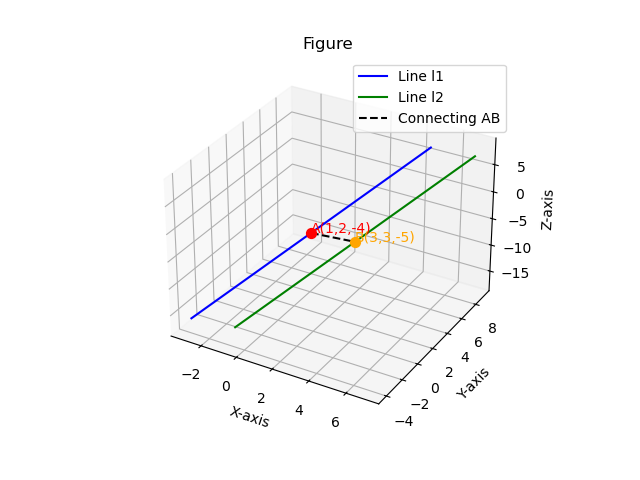
\includegraphics[height=0.5\textheight, keepaspectratio]{figs/figure1.png}
    \label{figure_1}
\end{figure}

\end{document}